\chapter{Diseño y modelado}

\section{Arquitectura}
ALTEM es una aplicación web de Stack Completo la cual está compuesta por las siguientes tecnologías
\begin{itemize}
    \item Front-End: Javascript ES5 con AngularJS 1.6
    \item BackE-End: PHP 7.1 con Laravel.
    \item Bases de Datos: SQL por MySQL.
\end{itemize}

Su API también se comunica con otros sistemas que pertenecen a la universidad, tales como

\begin{itemize}
    \item LDAP (Actualmente Deprecado)
    \item SAVIO (Moodle)
    \item Banner (Oracle)
\end{itemize}

En la Figura 3.1 Se puede apreciar la Arquitectura de ALTEM y la relacion existente entre cada uno de los elementos del stack y las APIs externas. 

\begin{figure}[H]
    \centering
    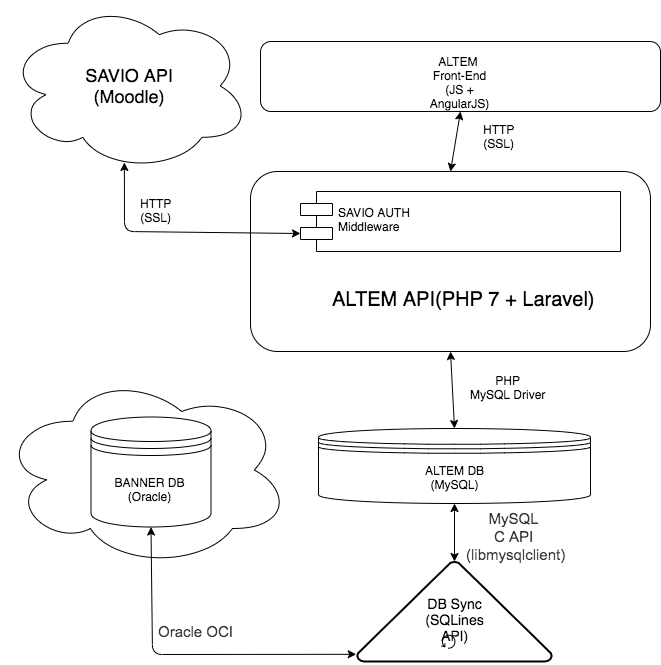
\includegraphics[width=0.7\textwidth]{img/ALTEM.png}
    \caption{Arquitectura de ALTEM}
\end{figure}

\subsection{Front-End}
Al ser una aplicacion web, ALTEM se consume desde el navegador, por medio de un Front-End creado en HTML5, CSS y JavaScript.

La capa de JavaScript está manejada por AngularJS 1.6, el cual nos facilita el desarrollo de las funcionalidades utilizando el patrón MVC el cual es un patrón de arquitectura de software, que separa los datos y la lógica de negocio de una aplicación de su representación, y el módulo encargado de gestionar los eventos y las comunicaciones.
MVC propone la construcción de tres componentes distintos que son el modelo, la vista y el controlador, es decir, por un lado define componentes para la representación de la información, y por otro lado para la interacción del usuario.\cite{trygve}

La aplicación web está compuesta por varios módulos, cada uno con sus modelos, vistas y controladores.

Los módulos son los siguientes:

\begin{itemize}
    \item Acción
    \item Estrategia
    \item Filtros
    \item Login
    \item Reportes
    \item Riesgos
    \item Tipos de Riesgos
    \item Usuarios
\end{itemize}

\subsubsection{Modelo}
Para el caso del cliente web, nuestro modelo equivale a todos los datos que vienen desde la API y que se solicitan por medio de peticiones HTTP. Estos datos se guardan en el localStorage y sessionStorage, y representan toda la información que el usuario puede ver a través de la vista en tiempo real.

Estas solicitudes a la API se encuentran organizadas en Servicios\cite{servicios} los cuales ejecutan llamadas a distintos endpoints\cite{endpoints}.

\begin{itemize}
    \item Acción
    \item Archivo Personal
    \item Criterio
    \item Estrategia
    \item Estudiante
    \item Filtro
    \item Intervención
    \item Login
    \item Observación
    \item Reporte
    \item Riesgo
    \item Tipo Riesgo
    \item Usuario
\end{itemize}

Estos servicios se comunican con el Back-End a trvés de la API de XMLHttpRequest(XHR) y utilizando métodos HTTP.

El Modelo es modificado por los Controladores, los cuales actualizan el estado de los datos dependiendo de las interacciones que tenga la aplicación con el usuario.
\subsubsection{Controlador}
Los controladores son funciones que disparan las instrucciones que modifican el Modelo, generalmente llamadas en la vista a través de eventos y en los servicios a través de Promesas.
En la aplicación web, todas las acciones (iniciar sesión, ver estudiantes, añadir estrategias, filtrar búsquedas, etc) disparan estos controladores, estos controladores se encuentran categorizados por los módulos mencionados en 1.1.

Las funciones principales de los controladores en la aplicación web son los siguientes:

\begin{itemize}
    \item Mutar el estado local de la aplicación.
    \item Hacer llamadas a los servicios.
    \item Actualizar la Vista.
\end{itemize}

Por lo general, las acciones ejecutadas en los controladores hacen que la vista se refresque.

\subsubsection{Vista}
La Vista se concibe como la capa presentacional de la aplicación web. Es la parte que interactúa con el usuario directamente y es la que se encarga de renderizar todos los datos del modelo en una manera que el usuario puede comprender fácilmente. 

Las vistas están hechas a través de plantillas HTML5 estilizadas con CSS, las cuales se renderizan de forma dinámica a medida que el modelo de la aplicación se actualice y se vayan ejecutando eventos que disparen los controladores.

La vista también se actualiza por medio de las directivas de AngularJS.

\subsection{Back-End}
El Back-End es el núcleo de ALTEM, consiste en una app Laravel y PHP7 en la que se encuentra toda la lógica del servidor.
Al igual que el Front-End, esta aplicación comparte la misma arquitectura MVC, pero orientada al lado del servidor. 

También, se encarga de comunicarse con API's de terceros como BANNER y SAVIO, plataformas pertenencientes a los recursos tecnológicos de la Universidad Tecnológica de Bolívar para obtener datos escenciales para su funcionamiento, de los cuales hablaremos más adelante. 




\subsection{Herramientas}
    \begin{itemize}
         \item JavaScript
         \item React native
    \end{itemize}
 \subsection{Modelos de desarrollo}
     KANVAN

\section{Plan de trabajo}

\subsection{Prioridad A}
\begin{itemize}
 \item Autenticación de usuarios (Savio) (Moodle)
 \item Información del usuario (Savio)
    \begin{itemize}
         \item ID
         \item Foto
         \item Nombre completo
         \item ...
    \end{itemize}
 \item Visualización de contactos (Universidad)
  \begin{itemize}
         \item Web
         \item Twiter, facebook...
         \item Números telefónicos
         \item ...
    \end{itemize}
 \item Visualización de cursos (Savio)
   \begin{itemize}
         \item Información del profesor
         \item Tareas pendientes
         \item ...
    \end{itemize}
\end{itemize}


\subsection{Prioridad B}
\begin{itemize}
 \item Visualización de notas parciales (Banner)
 \item Visualización de horarios de clase (Banner)
 \begin{itemize}
        \item Nombre del curso
        \item Hora
        \item Lugar
         \item ...
    \end{itemize}
\end{itemize}

\subsection{Prioridad C}
\begin{itemize}
 \item Visualización mapa UTB (Imagen sobre API google maps)
 \item Centro de notificaciones
     \begin{itemize}
         \item Savio
         \item Web
         \item Academia
    \end{itemize}
\end{itemize}